\documentclass[11pt,oneside,a4paper]{report}
\usepackage[utf8]{vietnam}
\usepackage{amsmath, amssymb, latexsym, amscd, amsthm,amstext}
\usepackage{color, colortbl, xcolor}                 
\usepackage[unicode]{hyperref}  
\usepackage{anysize}							
\usepackage[top=3.5cm, bottom=3.0cm, left=3.5cm, right=2.0cm]{geometry}  % căn lề theo quy chuẩn
\usepackage{longtable}               
\usepackage{graphicx}
\usepackage{array}
\usepackage{placeins}[section]
\usepackage{algorithm}
\usepackage{algpseudocode}
%=============================
\usepackage{multicol}
\usepackage{enumerate}
\usepackage{sectsty}
\usepackage{titlesec}   
\usepackage{url}
\usepackage{xurl}

%%========================================
\renewcommand{\baselinestretch}{1.5}
\usepackage[font=small]{caption}
\usepackage{titlesec}
%%========================================
\theoremstyle{definition}
\newtheorem{nx}{Nhận xét}[section]
\newtheorem{dl}{Định lý}[section]
\newtheorem{bd}{Bổ đề}[section]
\newtheorem{dn}{Định nghĩa}[section]
\newtheorem{vd}{Ví dụ} [section]
\newtheorem{hq}{Hệ quả}[section]
\newtheorem{cy}{Chú ý}[section]
\newtheorem{bt}{Bài tập}
%=========================================
%\usepackage{utopia}
%=======================
\usepackage{fancyhdr}
\pagestyle{fancy}
\lhead{}
\chead{\thepage}
\rhead{}
\lfoot{}
\cfoot{}
\rfoot{}
\renewcommand{\headrulewidth}{0pt}
\renewcommand{\footrulewidth}{0pt}
% =========================================
\usepackage{indentfirst}
% Thụt vào đầu dòng
% Chọn thụt hay ko thụt đoạn nào đó cụ thể thì chèn lệnh \indent hay \noindent đằng trước.


\usepackage{listings}

\definecolor{codegreen}{rgb}{0,0.6,0}
\definecolor{codegray}{rgb}{0.5,0.5,0.5}
\definecolor{codepurple}{rgb}{0.58,0,0.82}
\definecolor{backcolour}{rgb}{0.95,0.95,0.92}

\lstdefinestyle{mystyle}{
	backgroundcolor=\color{backcolour},   
	commentstyle=\color{codegreen},
	keywordstyle=\color{magenta},
	numberstyle=\tiny\color{codegray},
	stringstyle=\color{codepurple},
	basicstyle=\ttfamily\footnotesize,
	breakatwhitespace=false,         
	breaklines=true,                 
	captionpos=b,                    
	keepspaces=true,                                                    
	showspaces=false,                
	showstringspaces=false,
	showtabs=false,                  
	tabsize=1
}
\usepackage{tikz} 
\usepackage{scrextend}
\usetikzlibrary{calc}

\pagestyle{plain}
% dinh nghia lai kieu description cho dep
\newcommand{\seq}[1]{\left<#1\right>}
\makeatletter
\def\ps@myheadings{%
	\def\@evenhead{\hfil\thepage\hfil}
	\def\@oddhead{\hfil\thepage\hfil}}
\makeatother 
%\pagestyle{plain}% so trag o cuoi,giua
%\pagestyle{myheadings} %so trang o giua,dau

%\usepackage{fancyhdr} % Đánh số trang ở trên, nằm giữa
\pagestyle{fancy}
\makeatletter
\renewcommand{\ps@plain}{
	\renewcommand{\@oddhead}{\textrm{\centerline{\thepage}}}
	\renewcommand{\@evenhead}{\@oddhead}
	\renewcommand{\@oddfoot}{}
	\renewcommand{\@evenfoot}{\@oddfoot}}

\pagestyle{plain}
\lstset{style=mystyle}

\makeatletter
% Reinsert missing \algbackskip
\def\algbackskip{\hskip-\ALG@thistlm}
\makeatother
\begin{document}
\pagenumbering{gobble}%tắt đánh số trang

%  ======================= BÌA  =======================
\begin{titlepage}
\begin{tikzpicture}[remember picture,overlay,inner sep=0,outer sep=0]
\draw[black!70!black,line width=4pt] ([xshift=-2cm,yshift=-2cm]current page.north east) coordinate (A)--([xshift=3.5cm,yshift=-2cm]current page.north west) coordinate(B)--([xshift=3.5cm,yshift=2cm]current page.south west) coordinate (C)--([xshift=-2cm,yshift=2cm]current page.south east) coordinate(D)--cycle;
\end{tikzpicture}
\begin{center}
\vspace{-1cm}
\fontsize{13pt}{13pt}\selectfont 
\textbf{TRƯỜNG ĐẠI HỌC QUY NHƠN}\\
\fontsize{15pt}{15pt}\selectfont 
\textbf{KHOA TOÁN VÀ THỐNG KÊ}\\
\vspace{-0.5cm}
——————————————
\end{center}
\vspace{10pt}
\begin{center}
\vspace{1.5cm}
\fontsize{15pt}{15pt}\selectfont 
\textbf{TIỂU LUẬN MÔN HỌC}\\
\fontsize{17pt}{15pt}\selectfont 
\textbf{LÝ THUYẾT TỐI ƯU}
\end{center}
\vspace{1cm}
\begin{flushleft}
\fontsize{14pt}{17pt}\selectfont  
\begin{center}
\fontsize{18pt}{17pt}\selectfont 
\textbf{ĐỀ TÀI}
\end{center}
\end{flushleft}

\begin{center}
\fontsize{22pt}{17pt}\selectfont 
\textbf{\textrm{THUẬT TOÁN TỐI ƯU ADAM}}
\end{center}
	
\vspace{1.5cm}
\begin{center}
\begin{table}[!htb]
\centering
\fontsize{14pt}{14pt}\selectfont 
\begin{tabular}{rl}	
	GVHD:& \textbf{TS. TRẦN NGỌC NGUYÊN} \\
	HỌC VIÊN:& \textbf{NGUYỄN QUỐC DƯƠNG} \\
		MÃ SỐ HỌC VIÊN: & 8242548005\\
	LỚP:& KHOA HỌC DỮ LIỆU ỨNG DỤNG K24B\\
\end{tabular}
\end{table}
\end{center}
\vfill
\begin{center}
{\bf\fontsize{14pt}{16}\selectfont{Bình Định - Năm 2022}}
\end{center}
\end{titlepage}
%  ======================= MỤC LỤC =======================

\tableofcontents
\newpage
%\pagenumbering{roman}
\pagenumbering{arabic}
%  ======================= NỘI DUNG CHƯƠNG 1 =======================
\chapter{Kiến thức chuẩn bị}
\section{Giới thiệu tổng quan về tối ưu trong học sâu}

Các thuật toán tối ưu trong huấn luyện các mô hình đa tầng khác các thuật toán tối ưu thuần túy trên nhiều phương diện. Tối ưu trong học máy thường là tối ưu gián tiếp. Trong học máy, ta thường quan tâm đến một độ đo hiệu năng $P$ nào đó, được đánh giá trên tập kiểm thử và có thể có chi phí tính toán lớn. Do đó, ta chỉ tối ưu $P$ một cách gián tiếp. Chúng ta cố gắng làm giảm một hàm mất mát khác $J(\theta)$ và hi vọng điều đó sẽ cải thiện $P$. Điều này trái ngược với bài toán tối ưu thuần túy, ở đó cực tiểu hóa $J$ là hàm mục tiêu duy nhất. Các thuật toán tối ưu trong huấn luyện mô hình đa tầng thường bao gồm những đặc tính chuyên biệt tương ứng với những cấu trúc cụ thể của các hàm mục tiêu \cite{1}.

Các thuật toán học sâu cần giải quyết nhiều bài toán tối ưu trong nhiều ngữ cảnh. Ta thường dùng tối ưu dạng giải tích để chứng minh lí thuyết hoặc thiết kế các thuật toán. Trong tất cả các bài toán tối ưu liên quan đến học sâu, bài toán thách thức nhất là huấn luyện mạng neuron. Chúng ta thường phải chạy các thuật toán huẩn luyện mạng neuron trên nhiều máy tính trong một vài ngày hay thậm chí là vài tháng chỉ để huấn luyện một mạng neuron. Do tối ưu trong học sâu rất quan trọng và tốn kém, người ta đã phát triển riêng một tập các kĩ thuật tối ưu chuyên biệt để giải quyết các bài toán này \cite{1}.

Nhìn chung, các phương pháp học máy đã tránh những khó khăn trong tối ưu bằng cách thiết kế hàm mục tiêu và các ràng buộc cẩn thận sao cho bài toán tối ưu có tính lồi. Khi huấn luyện mạng neuron, chúng ta phải đối mặt với các trường hợp không lồi tổng quát. Ngay cả tối ưu lồi cũng có vấn đề của riêng nó. Một số thách thức điển hình nhất liên quan đến khâu tối ưu trong các mô hình huấn luyện đa tầng có thể kể đến như \textit{tính kém điều hòa} (coditioning); \textit{cực tiểu cục bộ} (local minima); \textit{cao nguyên, điểm yên ngựa và các vùng phẳng khác} (plateaus, saddle points and other flat regions); \textit{vách đứng và bùng nổ gradient} (cliffs and exploding gradients); \textit{phụ thuộc dài hạn} (long-term dependencies); \textit{gradient không chính xác} (inexact gradients); \textit{sự liên đới yếu giữa cấu trúc cục bộ và cấu trúc toàn cục} (poor correspondence between local and global structure). Những thuật ngữ này được trình bày chi tiết trong tài liệu số \cite{1,2}.

\section{Một số thuật toán tối ưu}
\subsection{Gradient Descent đa biến}
Với $\mathbf{x} \in \mathbb{R}^d$, hàm mục tiêu $f: \mathbb{R}^d \to \mathbb{R}$ ánh xạ các vector tới các giá trị vô hướng \cite{3}. Gradient tương ứng cũng là đa biến, là một vector gồm  $d$ đạo hàm riêng
$$\nabla f(\mathbf{x}) = \bigg[\frac{\partial f(\mathbf{x})}{\partial x_1}, \frac{\partial f(\mathbf{x})}{\partial x_2}, \ldots, \frac{\partial f(\mathbf{x})}{\partial x_d}\bigg]^\top.$$

Mỗi đạo hàm riêng $\partial f(\mathbf{x})/\partial x_i$ trong gradient biểu diễn tốc độ thay đổi theo $x_i$ của  $f$  tại $\mathbf{x}$. Sử dụng khai triển Taylor tương ứng cho các hàm đa biến, ta được
$$f(\mathbf{x} + \mathbf{\epsilon}) = f(\mathbf{x}) + \mathbf{\epsilon}^\top \nabla f(\mathbf{x}) + \mathcal{O}(\|\mathbf{\epsilon}\|^2).$$
Nói cách khác, chiều giảm mạnh nhất được cho bởi gradient âm $-\nabla f(\mathbf{x})$,  các hạng tử từ bậc hai trở lên trong $\mathbf{\epsilon}$ có thể bỏ qua. Chọn một tốc độ học phù hợp $\eta > 0$, ta được thuật toán gradient descent nguyên bản như sau
$$\mathbf{x} \leftarrow \mathbf{x} - \eta \nabla f(\mathbf{x}).$$
\subsubsection{Ưu điểm}
\begin{itemize}
\item Thuật toán gradient descent cơ bản, dễ hiểu. Thuật toán đã giải quyết được vấn đề tối ưu model neural network bằng cách cập nhật trọng số sau mỗi vòng lặp.
\end{itemize}
\subsubsection{Nhược điểm}
\begin{itemize}
\item Vì đơn giản nên thuật toán Gradient Descent còn nhiều hạn chế như phụ thuộc vào nghiệm khởi tạo ban đầu và learning rate.
\item Ví dụ 1 hàm số có 2 global minimum thì tùy thuộc vào 2 điểm khởi tạo ban đầu sẽ cho ra 2 nghiệm cuối cùng khác nhau.
\item Tốc độ học quá lớn sẽ khiến cho thuật toán không hội tụ, quanh quẩn bên đích vì bước nhảy quá lớn; hoặc tốc độ học nhỏ ảnh hưởng đến tốc độ training.
\end{itemize}
\subsection{Stochastic Gradient Descent}
\begin{figure}[!h]
	\centering
	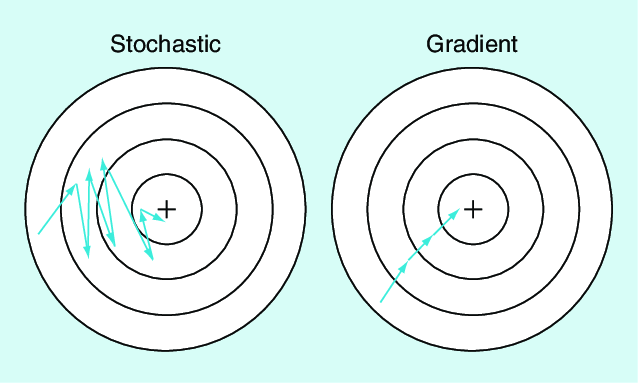
\includegraphics[scale=0.5]{images/h3}
	\caption{So sánh Gradient Descent với Stochastic Gradient Descent}
	\label{gdd}
\end{figure}

Trong học sâu, hàm mục tiêu thường là trung bình của các hàm mất mát cho từng mẫu trong tập huấn luyện. Giả sử tập huấn luyện có $n$  mẫu, $f_i(\mathbf{x})$ là hàm mất mát của mẫu thứ $i$  và vector tham số là $\mathbf{x}$.  Ta có hàm mục tiêu
$$f(\mathbf{x}) = \frac{1}{n} \sum_{i = 1}^n f_i(\mathbf{x}).$$
Gradient của hàm mục tiêu tại $\mathbf{x}$ được tính như sau
$$\nabla f(\mathbf{x}) = \frac{1}{n} \sum_{i = 1}^n \nabla f_i(\mathbf{x}).$$
Nếu gradient descent được sử dụng, chi phí tính toán cho mỗi vòng lặp độc lập là $\mathcal{O}(n)$, tăng tuyến tính với $n$. Do đó, với tập huấn luyện lớn, chi phí của gradient descent cho mỗi vòng lặp sẽ rất cao \cite{3}.

Hạ gradient ngẫu nhiên (stochastic gradient descent - SGD) giúp giảm chi phí tính toán ở mỗi vòng lặp. Ở mỗi vòng lặp, ta lấy ngẫu nhiên một mẫu dữ liệu có chỉ số $i\in\{1,\ldots, n\}$  theo phân phối đều, và chỉ cập nhật $\mathbf{x}$   bằng gradient $\nabla f_i(\mathbf{x})$:
$$\mathbf{x} \leftarrow \mathbf{x} - \eta \nabla f_i(\mathbf{x}).$$
Ở đây,  $\eta$ là tốc độ học.  Ta có thể thấy rằng chi phí tính toán cho mỗi vòng lặp giảm từ $\mathcal{O}(n)$  của hạ gradient xuống còn hằng số $\mathcal{O}(1)$. Hơn nữa, gradient ngẫu nhiên  $\nabla f_i(\mathbf{x})$  là một ước lượng không thiên lệch (\textit{unbiased}) của gradient $\nabla f(\mathbf{x})$
$$\mathbb{E}_i \nabla f_i(\mathbf{x}) = \frac{1}{n} \sum_{i = 1}^n \nabla f_i(\mathbf{x}) = \nabla f(\mathbf{x}).$$
Do đó, gradient ngẫu nhiên là một ước lượng gradient tốt.

Quan sát hình \ref{gdd}, ta thấy SGD có đường đi khá là zig zắc, không mượt như GD. Tuy nhiên, một điểm dữ liệu không thể đại diện cho toàn bộ dữ liệu. Chính vì lí do đó, GD có hạn chế đối với cơ sở dữ liệu lớn (vài triệu dữ liệu) thì việc tính toán đạo hàm trên toàn bộ dữ liệu qua mỗi vòng lặp trở nên cồng kềnh. Bên cạnh đó GD không phù hợp với online learning. 
\subsection{Momentum}
\begin{figure}[!h]
\centering
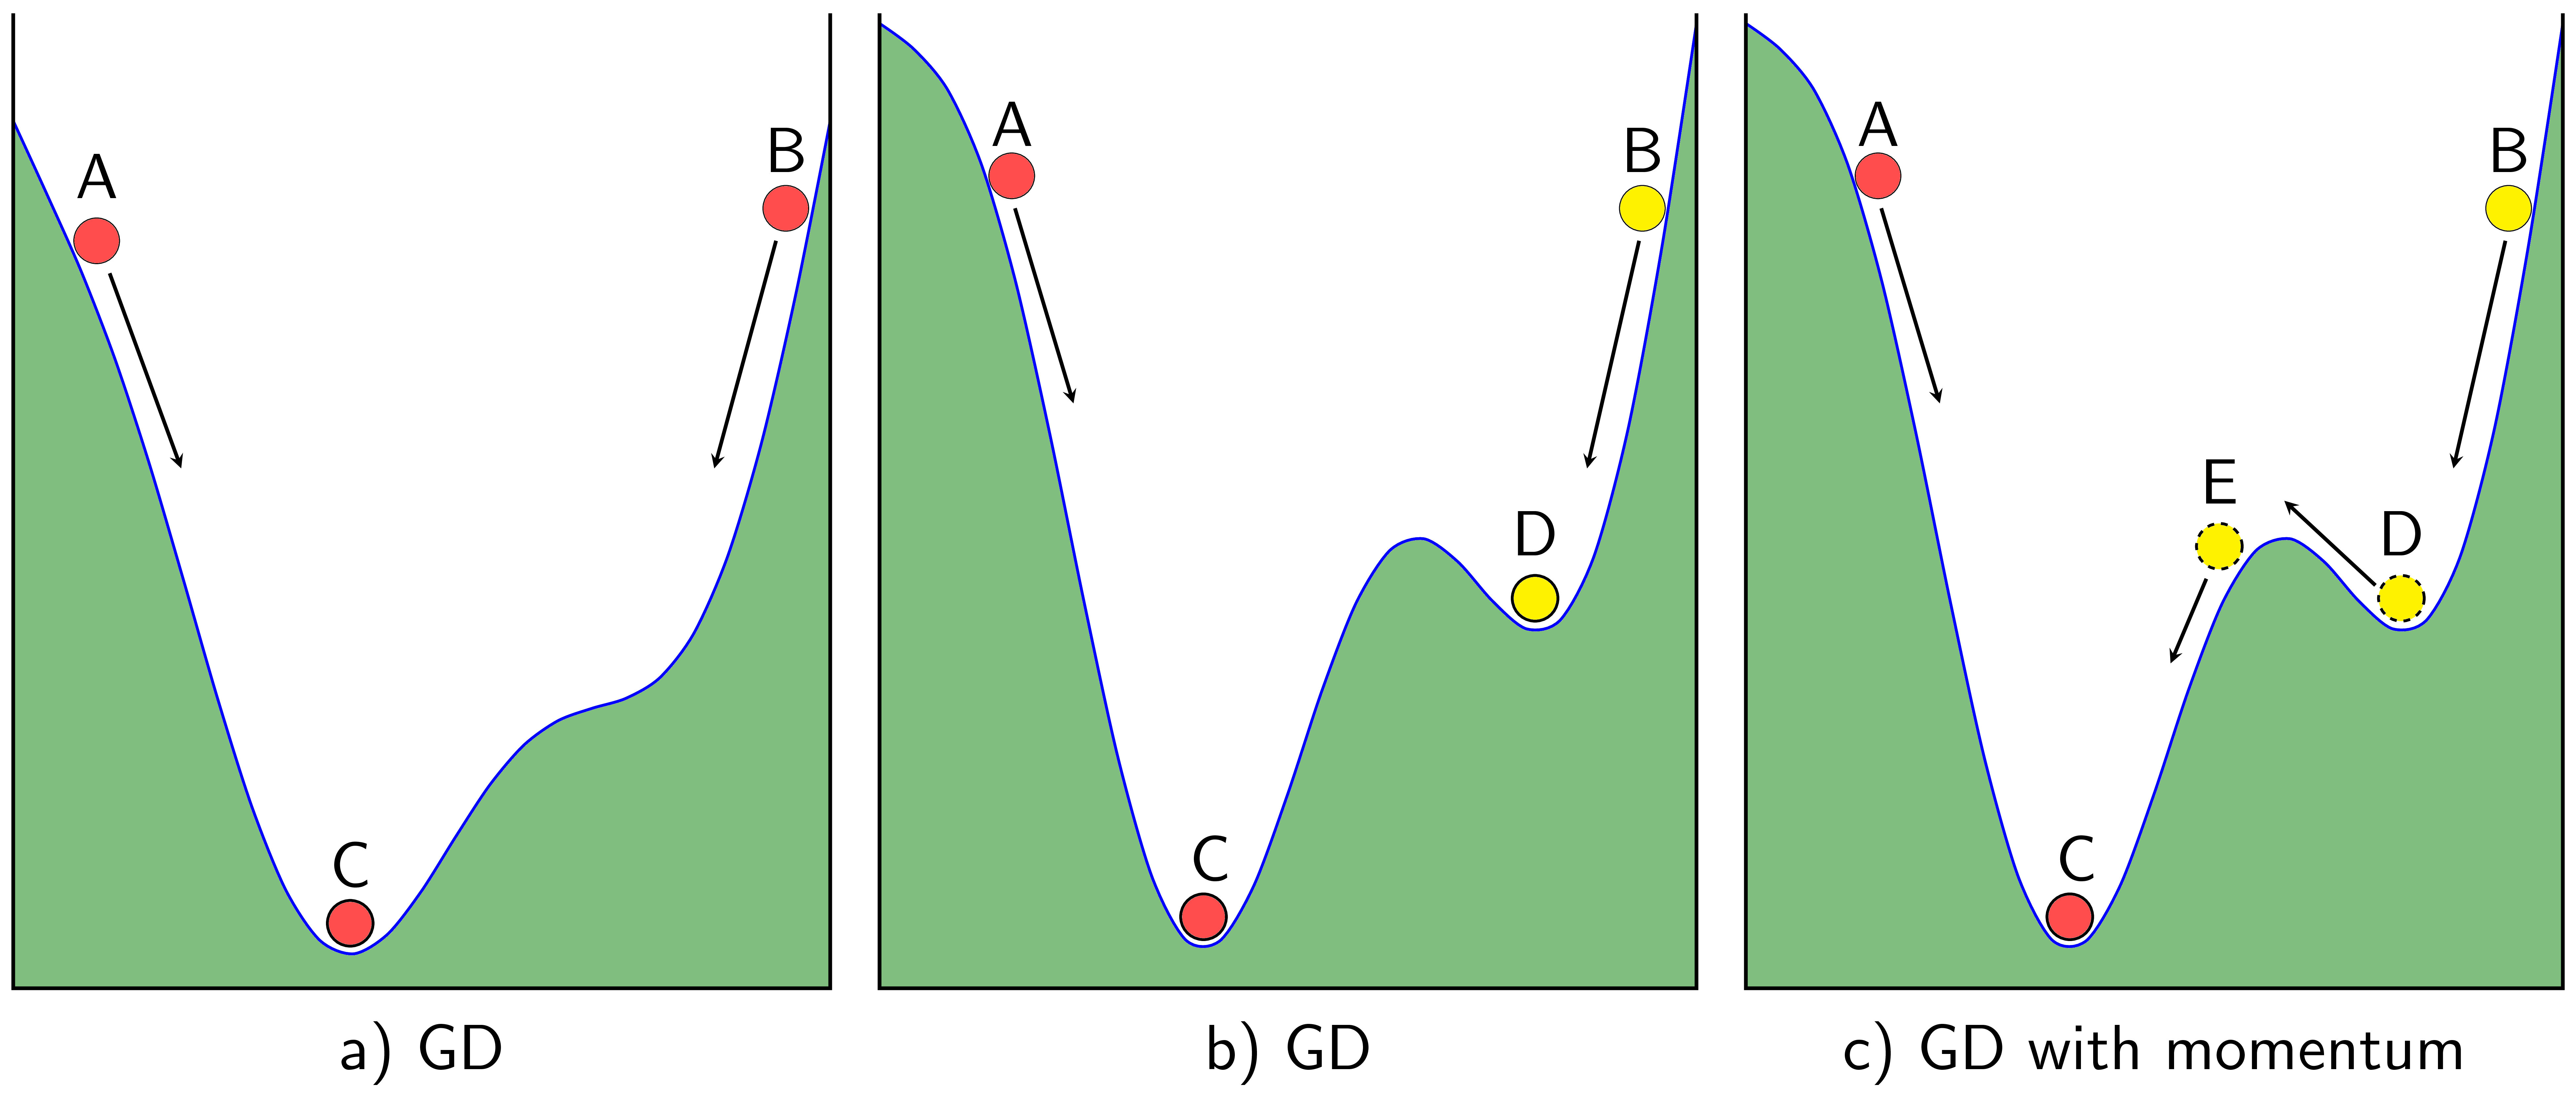
\includegraphics[scale=0.05]{images/h4}
\caption{So sánh Gradient Descent với các hiện tượng vật lý}
\label{olllolll}
\end{figure}
Một vấn đề đặt ra là khi có nhiễu ta cần chọn tốc độ học như thế nào để phù hợp. Nếu ta giảm tốc độ học quá nhanh, việc hội tụ sẽ ngưng trệ. Nếu tốc độ học giảm chậm, sẽ khó hội tụ tại một kết quả đủ tốt vì nhiễu sẽ đẩy điểm hội tụ ra xa điểm tối ưu. Để khắc phục các hạn chế trên của thuật toán Gradient Descent, người ta dùng gradient descent với momentum \cite{4}. 

\subsubsection{Ví dụ minh họa dưới góc nhìn vật lý}
Thuật toán GD thường được ví với tác dụng của trọng lực lên một hòn bi đặt trên một mặt có dạng như hình một thung lũng giống như hình \ref{olllolll}a. Bất kể ta đặt hòn bi ở A hay B thì cuối cùng hòn bi cũng sẽ lăn xuống và kết thúc ở vị trí C. Tuy nhiên, nếu như bề mặt có hai đáy thung lũng như Hình \ref{olllolll}b thì tùy vào việc đặt bi ở A hay B, vị trí cuối cùng của bi sẽ ở C hoặc D. Điểm D là một điểm local minimum chúng ta không mong muốn.

Nếu suy nghĩ một cách vật lý hơn, vẫn trong Hình \ref{olllolll}b, nếu vận tốc ban đầu của bi khi ở điểm B đủ lớn, khi bi lăn đến điểm D, theo đà, bi có thể tiếp tục di chuyển lên dốc phía bên trái của D. Và nếu giả sử vận tốc ban đầu lớn hơn nữa, bi có thể vượt dốc tới điểm E rồi lăn xuống C như trong Hình \ref{olllolll}c. Đây chính là điều chúng ta mong muốn. Bạn đọc có thể đặt câu hỏi rằng liệu bi lăn từ A tới C có theo đà lăn tới E rồi tới D không. Xin trả lời rằng điều này khó xảy ra hơn vì nếu so với dốc DE thì dốc CE cao hơn nhiều. Dựa trên hiện tượng này, thuật toán momentum được ra đời nhằm khắc phục việc nghiệm của GD rơi vào một điểm local minimum không mong muốn \cite{4, 5}.
\subsubsection{Biểu diễn momentum bằng toán học}
Trong GD, chúng ta cần tính lượng thay đổi ở thời điểm $t$ để cập nhật vị trí mới cho nghiệm (tức \textit{hòn bi}). Nếu chúng ta coi đại lượng này như vận tốc $v_t$ trong vật lý, vị trí mới của \textit{hòn bi} sẽ là $\theta_{t+1} = \theta_{t} - v_t$. Dấu trừ thể hiện việc phải di chuyển ngược với đạo hàm. Công việc của chúng ta bây giờ là tính đại lượng $v_t$ sao cho nó vừa mang thông tin của \textit{độ dốc} (tức đạo hàm), vừa mang thông tin của \textit{đà}, tức vận tốc trước đó $v_{t-1}$ (chúng ta coi như vận tốc ban đầu $v_0=0$). Một cách đơn giản nhất, ta có thể cộng (có trọng số) hai đại lượng này lại, ta được 
\begin{equation} 
v_{t}= \gamma v_{t-1} + \eta \nabla_{\theta}J(\theta) .
\end{equation} 

Trong đó $\gamma$ thường được chọn là một giá trị khoảng 0.9, $v_t$ là vận tốc tại thời điểm trước đó, $ \nabla_{\theta}J(\theta)$ chính là độ dốc của điểm trước đó.  
Sau đó vị trí mới của \textit{hòn bi} được xác định như sau
\begin{equation} 
\theta = \theta - v_t .
\end{equation} 
\subsubsection{Ưu điểm}
Thuật toán tối ưu giải quyết được vấn đề: Gradient Descent không tiến được tới điểm global minimum mà chỉ dừng lại ở local minimum.
\subsubsection{Nhược điểm}
Tuy momentum giúp hòn bi vượt dốc tiến tới điểm đích, tuy nhiên khi tới gần đích, nó vẫn mất khá nhiều thời gian giao động qua lại trước khi dừng hẳn, điều này được giải thích vì viên bi có đà.

\subsection{Adagrad}
Thuật toán Adagrad điều chỉnh tốc độ học của toàn bộ tham số mô hình một cách riêng biệt bằng cách chia chúng cho nghịch đảo căn bậc hai của tổng toàn bộ các bình phương gradient trong quá khứ. Các tham số có đạo hàm riêng của hàm mất mát càng lớn thì các tốc độ học tương ứng càng giảm nhanh, trong khi những tham số có đạo hàm riêng nhỏ sẽ có tốc độ giảm chậm tương ứng. Hệ quả là thuật toán sẽ học nhanh hơn ở những hướng có độ dốc nhỏ hơn trong không gian tham số. Tuy nhiên, khi huấn luyện các mô hình mạng neuron đa tầng, việc tích lũy các bình phương gradient ngay từ khi bắt đầu quá trình huấn luyện có thể làm giảm tốc độ học quá sớm và quá mức cần thiết \cite{1,6}.
\subsection{RMSProp}
Thuật toán RMSProp là một phiên bản sửa đổi của AdaGrad để hoạt động tốt hơn với các bài toán tối ưu không lồi bằng cách tích lũy gradient vào một trung bình động lũy thừa có trọng số. AdaGrad được thiết kế để hội tụ nhanh chóng khi được áp dụng cho một hàm lồi.

RMSprop giải quyết vấn đề tỷ lệ học giảm dần của Adagrad bằng cách chia tỷ lệ học cho trung bình của bình phương gradient.
$$
\begin{aligned}
E\left[g^2\right]_t &=0,9 E\left[g^2\right]_{t-1}+0,1 g_t^2, \\
\theta_{t+1} &=\theta_t-\frac{\eta}{\sqrt{E\left[g^2\right]_t+\epsilon}} g_t.
\end{aligned}
$$

Khi được áp dụng cho hàm không lồi để huấn luyện mạng neuron thì quỹ đạo của quá trình học có thể bỏ qua nhiều cấu trúc và cuối cùng tiến đến một vùng lồi cục bộ. Adagrad giảm dần tốc độ học theo toàn bộ giá trị bình phương gradient trong quá khứ và có thể khiến tốc độ học trở nên quá nhỏ trước khi đến được một cấu trúc lồi. RMSProp sử dụng một trung bình động lũy thừa giảm để loại bỏ các dữ kiện từ quá khứ quá xa, giúp nó có thể hội tụ nhanh chóng sau khi tìm thấy vùng lồi, như thể đó là một trường hợp khi thuật toán AdaGrad được khởi tạo bên trong vùng lồi đó \cite{1}.

Qua thực nghiệm, RMSProp tỏ ra là một thuật toán tối ưu hiệu quả và thực dụng đối với các mạng neuron đa tầng. Nó đang là một trong những phương pháp tối ưu mà các chuyên gia học sâu áp dụng thường xuyên.
\subsubsection{Ưu điểm}
Ưu điểm rõ nhất của RMSprop là giải quyết được vấn đề tốc độ học giảm dần của Adagrad (vấn đề tốc độ học giảm dần theo thời gian sẽ khiến việc training chậm dần, có thể dẫn tới bị đóng băng).
\subsubsection{Nhược điểm}
Thuật toán RMSprop có thể cho kết quả nghiệm chỉ là local minimum chứ không đạt được global minimum như Momentum.
\chapter{Thuật toán tối ưu Adam}
\begin{algorithm}[!h]
	\caption{Thuật toán Adam. Kí hiệu $g_t^2$ là bình phương của phép nhân element-wise $g_t\odot g_t$, các tham số khuyến nghị là $\alpha = 0.001, \beta_1 = 0.9, \beta_2 = 0.999$ và $\varepsilon = 10^{-8}$. Tất cả các toán tử trên vector là phép element-wise (tức là thực hiện tương ứng từng phần tử).} 
	\begin{algorithmic}
		\Require $\alpha$: Độ lớn mỗi bước.
		\Require $\beta_1, \beta_2 \in [0,1)$: Tốc độ suy giảm theo hàm mũ của các ước lượng moment.
		\Require $f(\theta)$: Stochastic objective function with parameters $\theta$.
		\Require $\theta_0$: Tham số khởi tạo.
		\State $m_0 \leftarrow 0$  (Khởi tạo moment bậc 1).
		\State $v_0 \leftarrow 0$ (Khởi tạo moment bậc 2).
		\State $t \leftarrow 0$ (Khởi tạo thứ tự bước $t$.)
		\While{$\theta_0$ not converged} 
		\State $t \leftarrow t+1$
		\State $g_t \leftarrow \nabla_\theta f_t\left(\theta_{t-1}\right)$ (Tính gradient tại mỗi bước $t$). 
		\State $m_t \leftarrow \beta_1 \cdot m_{t-1}+\left(1-\beta_1\right) \cdot g_t$ (Cập nhật giá trị moment bậc 1). 
		\State $v_t \leftarrow \beta_2 \cdot v_{t-1}+\left(1-\beta_2\right) \cdot g_t^2$ (Cập nhật giá trị moment bậc 2). 
		\State $\widehat{m}_t \leftarrow m_t /\left(1-\beta_1^t\right)$ (Hiệu chỉnh độ chệch trong moment bậc 1).
		\State $\widehat{v}_t \leftarrow v_t /\left(1-\beta_2^t\right)$ (Hiệu chỉnh độ chệch trong moment bậc 2).
		\State $\theta_t \leftarrow \theta_{t-1}-\alpha \cdot \widehat{m}_t /\left(\sqrt{\widehat{v}_t}+\epsilon\right)$ (Cập nhật các tham số.)
		\EndWhile\\
		\Return $\theta_t$ (Resulting parameters).
	\end{algorithmic}
\end{algorithm}
\section{Phân tích và đánh giá thuật toán}
Adam (Adaptive moment Estimation) là một thuật toán tối ưu tự điều chỉnh tốc độ học \cite{7}. Cái tên "Adam" bắt nguồn từ cụm từ "adaptive moment" (moment thích nghi). Adam được coi như là sự kết hợp giữa RMSProp và momentum. Trong khi momentum có thể xem như một quả bóng đang chạy xuống dốc, Adam lại giống như một quả bóng nặng với ma sát. Adam sử dụng bình phương gradient để chia tỷ lệ learning rate như RMSProp và tận dụng "đà" giống như momentum. Adam tính toán moment cấp 1 và moment cấp 2 của gradient để ước lượng learning rate cho các tham số. Công thức cập nhật đầy đủ của Adam
\begin{align}
\begin{cases}
m_t= \beta_1 \cdot m_{t-1}+\left(1-\beta_1\right) \cdot g_t,\\
v_t= \beta_2 \cdot v_{t-1}+\left(1-\beta_2\right) \cdot g_t^2,\\
\hat{m}_t=\dfrac{m_t}{1-\beta_1^t} ,\\
\hat{v}_t=\dfrac{v_t}{1-\beta_2^t} ,\\
\theta_t=\theta_{t-1}-\eta \dfrac{\hat{m}t}{\sqrt{\hat{v}_t}+\varepsilon}.
\label{eq1}
\end{cases}
\end{align}
Để tốt hơn về chi phí tính toán,  chúng ta có thể viết lại 3 phương trình cuối trong hệ phương trình \ref{eq1} như sau 
\begin{align}
\eta_t&=\eta \dfrac{\sqrt{1-\beta_2^t}}{1-\beta_1^t}, \\
\theta_t&=\theta_{t-1}-\eta_t \dfrac{m_t}{\sqrt{v_t}+\varepsilon}.
\end{align}

\begin{dn}[Khái niệm moment]
Moment cấp $k$ đối với $a$ của biến ngẫu nhiên $X$ là một số xác định như sau
$$
v_k(a)=E\left[(X-a)^k\right].
$$
Nếu $a=0$, ta ký hiệu $v_k=v_k(0)=E\left(X^k\right)$ và gọi nó là moment gốc cấp $k$. Rõ ràng kỳ vọng chính là moment gốc cấp 1 ($E X=v_1$). Nếu $a=E X$, ta ký hiệu $\mu_k=v_k(E X)=$ $E\left[(X-E X)^k\right]$ và gọi nó là moment trung tâm cấp $k$. Hơn nữa, phương sai là moment trung tâm cấp 2 ($V X=\mu_2$). Người ta còn dùng moment để đặc trưng cho hình dạng của mật độ phân phối.
\end{dn}

Như đã thấy ở thuật toán, Adam sử dụng thuật ngữ khởi tạo \textit{bias correction}. Chúng ta sẽ làm rõ điều này cho ước lượng moment cấp 2, nguồn gốc ước lượng moment cấp 1 là tương tự.
Ta thấy rằng, gradient của hàm mục tiêu có thể xem như là một biến ngẫu nhiên, vì nó thường được đánh giá trên một mini-batch dữ liệu. Moment cấp 1 là kỳ vọng, moment cấp 2 là \textit{uncentered variance} (Có nghĩa là moment gốc cấp 2 - chúng ta không trừ đi giá trị trung bình khi tính toán phương sai). Adam tận dụng \textit{exponentially moving average} của gradient và bình phương gradient để ước lượng các moment như sau
$$
\begin{aligned}
m_t &=\beta_1 m_{t-1}+\left(1-\beta_1\right) g_t, \\
v_t &=\beta_2 v_{t-1}+\left(1-\beta_2\right) g_t^2.
\end{aligned}
$$
Trong đó \textit{decay rate} là $\beta_1$ và $\beta_2$; $m_t$ và $v_t$ được gọi là moving averages, $g$ là gradient trên mini-batch hiện tại. Để xem các giá trị này tương quan với moment như thế nào, chúng ta hãy xem xét giá trị kỳ vọng của các moving averages. Vì $m$ và $v$ là các uớc lượng của moment cấp 1 và moment cấp 2, chúng ta muốn có tính chất sau
$$
\begin{aligned}
&\mathbb{E}\left[m_t\right]=\mathbb{E}\left[g_t\right],\\
&\mathbb{E}\left[v_t\right]=\mathbb{E}\left[g_t^2\right].
\end{aligned}
$$
Ta khai triển $v_t$ như sau (tương tự với $m_t$ ):
$$
\begin{aligned}
v_0 &=0, \\
v_1 &=\beta_2 v_0+\left(1-\beta_2\right) g_1^2=\left(1-\beta_2\right) g_1^2 ,\\
v_2 &=\beta_2 v_1+\left(1-\beta_2\right) g_2^2=\beta_2\left(1-\beta_2\right) g_1^2+\left(1-\beta_2\right) g_2^2,\\
&\vdots\\
v_t &=\beta_2 v_{t-1}+\left(1-\beta_2\right) g_t^2=\left(1-\beta_2\right) \sum_{i=1}^t \beta_2^{t-i} \cdot g_i^2.
\end{aligned}
$$
Do $\beta_2 \in[0,1)$ nên ta có thể thấy rằng exponential moving average đánh trọng số cho các gradient, các gradient đầu tiên thì đóng góp ít vào giá trị tổng thể, vì chúng được nhân với $\beta$ nhỏ hơn. Bây giờ chúng ta sẽ xem xét giá trị kỳ vọng của $v_t$ để xem nó liên quan thế nào đến giá trị thực moment cấp 2 là $\mathbb{E}\left[g_t^2\right]$. Ta có
$$
\begin{aligned}
\mathbb{E}\left[v_t\right] &=\mathbb{E}\left[\left(1-\beta_2\right) \sum_{i=1}^t \beta_2^{t-i} \cdot g_i^2\right] \\
&=\mathbb{E}\left[g_t^2\right] \cdot\left(1-\beta_2\right) \sum_{i=1}^t \beta_2^{t-i}+\zeta \\
&=\mathbb{E}\left[g_t^2\right] \cdot\left(1-\beta_2^t\right)+\zeta.
\end{aligned}
$$
Ở khai triển trên, chúng ta đã sử dụng xấp xỉ $g_i$ thành $g_t$ và đưa nó ra khỏi tổng. Vì sự xấp xỉ này nên ta cần cộng thêm một đại lượng $\zeta$ trong công thức để đại diện cho sai lệch do xấp xỉ. Tiếp theo, chúng ta cần điều chỉnh giá trị ước lượng của $v_t$ để cho kỳ vọng của nó xấp xỉ moment cấp 2. Sự sai lệch đại lượng $\left(1-\beta_2^t\right)$ là do ta đã khởi tạo $v_0=0$. Từ đó, chúng ta có công thức hiệu chỉnh cho $v$ như sau
$$
\hat{v_t}=\dfrac{v_t}{1-\beta_2^t}.
$$
Tương tự, thực hiện các bước trên với $m_t$. Cuối cùng, chúng ta có công thức cập nhật tham số cho Adam như sau
$$
\theta_t=\theta_{t-1}-\eta \dfrac{\hat{m}_t}{\sqrt{\hat{v}_t}+\varepsilon}.
$$
\section{Đánh giá sự hội tụ}
\subsection{Sai lầm trong chứng minh hội tụ của Kingma \& Ba}
Trong bài báo gốc về thuật toán Adam \cite{7}, Kingma và Lei Ba đã có những sai lầm trong phân tích sự hội tụ của thuật toán Adam. Sau đây, chúng ta sẽ cùng phân tích lỗi sai của họ.

Gọi $f_1(\theta), f_2(\theta), \ldots, f_T(\theta)$ là một dãy các hàm chi phí và lồi tại vòng lặp tương ứng $1,2, \ldots, T$.
Đặt $g_t:=\nabla f_t\left(\theta_t\right)$ và gọi $g_{t, i}$ là phần tử thứ $i$ của vector gradient $g_t$.
Đặt $g_{1: t, i}=\left[g_{1, i}, g_{2, i}, \ldots, g_{t, i}\right] \in \mathbb{R}^t$ và $\gamma:=\dfrac{\beta_1^2}{\sqrt{\beta_2}}$.
Gọi $\theta^*$ là tham số tối ưu của bài toán, $\theta_t$ là tham số dự đoán được tại vòng lặp thứ $t$. Do đó, tổng sai lệch của mô hình qua $T$ vòng lặp là
$$
R(T)=\sum_{t=1}^T\left[f_t\left(\theta_t\right)-f_t\left(\theta^*\right)\right].
$$
Chúng ta cần chứng minh cận trên của $R(T)$ sẽ nhỏ hơn hoặc bằng $O(T)$ để từ đó có thể đánh giá được $\dfrac{R(T)}{T} \rightarrow C$ khi $T \rightarrow \infty$. Trong bài báo của Kingma và Lei Ba, các tác giả đã chứng minh và chỉ ra định lý sau.

\begin{dl}
Giả sử rằng các hàm $f_t$ có gradient bị chặn, $\left\|\nabla f_t(\theta)\right\|_2 \leq G,\left\|\nabla f_t(\theta)\right\|_{\infty} \leq G_{\infty}$ với mọi tham số $\theta \in \mathbb{R}^d$, và khoảng cách giữa 2 tham số $\theta_t$ bất kỳ được sinh ra bởi Adam là bị chặn, $\left\|\theta_n-\theta_m\right\|_2 \leq D,\left\|\theta_m-\theta_n\right\|_{\infty} \leq D_{\infty}$ với mọi $m, n$ bất kỳ thuộc $\{1, \ldots, T\}$, và $\beta_1, \beta_2 \in[0,1)$ thoả mãn $\dfrac{\beta_1^2}{\sqrt{\beta_2}}<1$. Đặt $\alpha_t=\dfrac{\alpha}{\sqrt{t}}$ và $\beta_{1, t}=\beta_1 \lambda^{t-1}, \lambda \in(0,1)$. Với mọi $T\geq1$, ta có
$$
R(T) \leq \dfrac{D^2}{2 \alpha\left(1-\beta_1\right)} \sum_{i=1}^d \sqrt{T \hat{v}_{T, i}}+\dfrac{\alpha\left(1+\beta_1\right) G_{\infty}}{\left(1-\beta_1\right) \sqrt{1-\beta_2}(1-\gamma)^2} \sum_{i=1}^d\left\|g_{1: T, i}\right\|_2+\sum_{i=1}^d \dfrac{D_{\infty}^2 G_{\infty} \sqrt{1-\beta_2}}{2 \alpha\left(1-\beta_1\right)(1-\lambda)^2}.
$$
\end{dl}
Từ định lý này, các tác giả kết luận được rằng $\dfrac{R(T)}{T}=O\left(\dfrac{1}{\sqrt{T}}\right)$. Từ đó, khi $T \rightarrow \infty$ thì $\dfrac{R(T)}{T} \rightarrow 0$ và hội tụ. Tuy nhiên, định lý trên là không chính xác vì các tác giả đã chứng minh sai các bổ đề trong bài báo. Các tác giả đã sử dụng các bổ đề được nêu ra sau đây.
\begin{bd}
Nếu một hàm $f: \mathbb{R}^d \rightarrow \mathbb{R}$ là lồi thì:
$$
f(y) \geq f(x)+\nabla f(x)^T(y-x),
$$
với $x, y \in \mathbb{R}^d$ và $\lambda \in[0,1]$.
\label{bd1}
\end{bd}
Bổ đề \ref{bd1} là một tính chất của hàm lồi, phổ biến và đã được chứng minh nhiều trong các tài liệu khác nên chúng ta thừa nhận kết quả này. Sau đây là chứng minh chi tiết của Kingma và Lei Ba và lỗi sai trong chứng minh các bổ đề của họ.
\begin{bd}
Giả sử $\left\|g_t\right\|_2 \leq G,\left\|g_t\right\|_{\infty} \leq G_{\infty}$, khi đó 
$$
\sum_{t=1}^T \sqrt{\dfrac{g_{t, i}^2}{t}} \leq 2 G_{\infty}\left\|g_{1: T, i}\right\|_2.
$$ \label{bd2}
\end{bd}
Sau đây, chúng ta sẽ chỉ ra bổ đề \ref{bd2} chưa chặt chẽ.

\begin{proof}
	Chúng ta sẽ chứng minh bằng phương pháp quy nạp.
	Với $T=1$, ta có $\sqrt{g_{1, i}^2}=\left|g_{1, i}\right| \leq G_{\infty}$.
	Tuy nhiên,i Kingma \& Ba đã đánh giá như sau
	$$
	\sqrt{g_{1, t}^2} \leq 2 G_{\infty}\left\|g_{1, i}\right\|_2.
	$$
	Rõ ràng, điều này chỉ đúng khi $G_{\infty} \geq 0.5$ và điều kiện này không được các tác giả đưa ra. Hơn nữa, bước chứng minh quy nạp cũng có một sai lầm khác trong bổ đề này.
	Giả sử bổ đề đúng với $T=K-1$, ta có
	$$
	\sum_{t=1}^{K-1} \sqrt{\dfrac{g_{t, i}^2}{t}} \leq 2 G_{\infty}\left\|g_{1: K-1, i}\right\|_2.
	$$
	Cần chứng minh bổ đề đúng với $T=K$:
	$$
	\begin{aligned}
	\sum_{t=1}^K \sqrt{\dfrac{g_{t, i}^2}{t}} &=\sum_{t=1}^{K-1} \sqrt{\dfrac{g_{t, i}^2}{t}}+\sqrt{\dfrac{g_{K, i}^2}{K}} \\
	& \leq 2 G_{\infty}\left\|g_{1: K-1, i}\right\|_2+\sqrt{\dfrac{g_{K, i}^2}{K}} \\
	&=2 G_{\infty} \sqrt{\sum_{t=1}^{K-1} g_{t, i}^2+g_{K, i}^2-g_{K, i}^2}++\sqrt{\dfrac{g_{K, i}^2}{K}} \\
	&=2 G_{\infty} \sqrt{\left\|g_{1: K, i}\right\|_2^2-g_{K, i}^2}+\sqrt{\dfrac{g_{K, i}^2}{K}}
	\end{aligned}
	$$
	Sử dụng bất đẳng thức
	$$
	\left\|g_{1: K, i}\right\|_2^2-g_{K, i}^2 \leq\left\|g_{1: K, i}\right\|_2^2-g_{K, i}^2+\dfrac{g_{K, i}^4}{4\left\|g_{1: K, i}\right\|_2^2}=\left(\left\|g_{1: K, i}\right\|_2-\dfrac{g_{K, i}^2}{2\left\|g_{1: K, i}\right\|_2}\right)^2.
	$$
	Từ đó
	$$
	\begin{aligned}
	\sum_{t=1}^K \sqrt{\dfrac{g_{t, i}^2}{t}} & \leq 2 G_{\infty}\left(\left\|g_{1: K, i}\right\|_2-\dfrac{g_{K, i}^2}{2\left\|g_{1: K, i}\right\|_2}\right)+\sqrt{\dfrac{g_{K, i}^2}{K}} \\
	& \leq 2 G_{\infty}\left(\left\|g_{1: K, i}\right\|_2-\dfrac{g_{K, i}^2}{2 \sqrt{K G_{\infty}^2}}\right)+\sqrt{\dfrac{g_{K, i}^2}{K}} \\
	&=2 G_{\infty}\left\|g_{1: K, i}\right\|_2-\dfrac{g_{K, i}^2}{\sqrt{K}}+\sqrt{\dfrac{g_{K, i}^2}{K}}
	\end{aligned}
	$$
	Trong chứng minh của Kingma \& Ba, họ đánh giá như sau
	$$
	2 G_{\infty}\left\|g_{1: K, i}\right\|_2-\dfrac{g_{K, i}^2}{\sqrt{K}}+\sqrt{\dfrac{g_{K, i}^2}{K}} \leq 2 G_{\infty}\left\|g_{1: T, i}\right\|_2.
	$$
	Nếu đẳng thức trên đúng, thì chứng minh theo quy nạp kết thúc. Tuy nhiên, không đảm bảo rằng đẳng thức trên sẽ đúng, đẳng thức trên tương đương với $g_{K, i}^2 \leq\left|g_{K, i}\right|$ chỉ đúng với $\left|g_{K, i}\right| \leq 1$. Do đó, bổ đề \ref{bd1} được dùng để chứng minh cho bổ đề \ref{bd2} là chưa chặt chẽ.
\end{proof}

\begin{bd} Giả sử $\gamma<1$ và $\left\|g_t\right\|_2 \leq G,\left\|g_t\right\|_{\infty} \leq G_{\infty}$, thì
$$
\sum_{t=1}^T \dfrac{\hat{m}_{t, i}^2}{\sqrt{t \hat{v}_{t, i}}} \leq \dfrac{2}{1-\gamma} \dfrac{1}{\sqrt{1-\beta_2}}\left\|g_{1: T, i}\right\|_2.
$$
\begin{proof}
Từ giả thiết, ta có $\dfrac{\sqrt{1-\beta_2^t}}{\left(1-\beta_1^t\right)^2} \leq \dfrac{1}{\left(1-\beta_1\right)^2}$. Khai triển vế trái, ta có
$$
\begin{aligned}
\sum_{t=1}^T \dfrac{\hat{m}_{t, i}^2}{\sqrt{t \hat{v}_{t, i}}} &=\sum_{t=1}^{T-1} \dfrac{\hat{m}_{t, i}}{\sqrt{t \hat{v}_{t, i}}}+\dfrac{\sqrt{1-\beta_2^T}}{\left(1-\beta_1^T\right)^2} \dfrac{\left(\sum_{k=1}^T\left(1-\beta_1\right) \beta_1^{T-k} g_{k, i}\right)^2}{\sqrt{T \sum_{j=1}^T\left(1-\beta_2\right) \beta_2^{T-j} g_{j, i}^2}} \\
& \leq \sum_{t=1}^{T-1} \dfrac{\hat{m}_{t, i}}{\sqrt{t \hat{v}_{t, i}}}+\dfrac{\sqrt{1-\beta_2^T}}{\left(1-\beta_1^T\right)^2} \sum_{k=1}^T \dfrac{T\left(\left(1-\beta_1\right) \beta_1^{T-k} g_{k, i}\right)^2}{\sqrt{T \sum_{j=1}^T\left(1-\beta_2\right) \beta_2^{T-j} g_{j, i}^2}} \\
& \leq \sum_{t=1}^{T-1} \dfrac{\hat{m}_{t, i}}{\sqrt{t \hat{v}_{t, i}}}+\dfrac{\sqrt{1-\beta_2^T}}{\left(1-\beta_1^T\right)^2} \sum_{k=1}^T \dfrac{T\left(\left(1-\beta_1\right) \beta_1^{T-k} g_{k, i}\right)^2}{\sqrt{T\left(1-\beta_2\right) \beta_2^{T-k} g_{k, i}^2}} \\
& \leq \sum_{t=1}^{T-1} \dfrac{\hat{m}_{t, i}}{\sqrt{t \hat{v}_{t, i}}}+\dfrac{\sqrt{1-\beta_2^T}}{\left(1-\beta_1^T\right)^2} \dfrac{\left(1-\beta_1\right)^2}{\sqrt{T\left(1-\beta_2\right)^2}} \sum_{k=1}^T T\left(\dfrac{\beta_1^2}{\sqrt{\beta_2}}\right)^{T-k}\left\|g_{k, i}\right\|_2 \\
& \leq \sum_{t=1}^{T-1} \dfrac{\hat{m}_{t, i}}{\sqrt{t \hat{v}_{t, i}}}+\dfrac{T}{\sqrt{T\left(1-\beta_2\right)}} \sum_{k=1}^T \gamma^{T-k}\left\|g_{k, i}\right\|_2.
\end{aligned}
$$
Tới đây, Kingma \& Ba đã chứng minh như sau
$$
\begin{aligned}
\sum_{t=1}^T \dfrac{\hat{m}_{t, i}^2}{\sqrt{t \hat{v}_{t, i}}} & \leq \sum_{t=1}^T \dfrac{\left\|g_{t, i}\right\|_2}{\sqrt{t\left(1-\beta_2\right)}} \sum_{j=0}^{T-t} t \gamma^j \\
& \leq \sum_{t=1}^T \dfrac{\left\|g_{t, i}\right\|_2}{\sqrt{t\left(1-\beta_2\right)}} \sum_{j=0}^T t \gamma^j.
\end{aligned}
$$
Điều này là không dễ dàng suy ra được. Rõ ràng, từ chứng mình trên, ta chỉ có thể đánh giá như sau
$$
\sum_{t=1}^T \dfrac{\hat{m}_{t, i}^2}{\sqrt{t \hat{v}_{t, i}}} \leq \sum_{t=1}^T \dfrac{t}{\sqrt{t\left(1-\beta_2\right)}} \sum_{k=1}^t \gamma^{t-k}\left\|g_{k, i}\right\|_2.
$$
Có lẽ các bước đánh giá sai bổ đề của Kingma \& Ba đã gây nhầm lẫn trong việc chứng minh hội tụ Adam.
\end{proof}
\end{bd}
\subsection{Chứng minh thuật toán Adam có thể không hội tụ}
Trong báo cáo của Sashank J. Reddi, Satyen Kate và Sanjiv Kumar tại ICLR 2018 \cite{8}, các tác giả đã chứng minh thuật toán Adam không hội tụ và đề xuất ra các mở rộng, cải tiến.
Trong phần này, chúng ta quy ước các kí hiệu:
\begin{itemize}
\item $\mathbb{S}_d^{+}$: tập tất cả các ma trận xác dịnh dương $d \times d$.
\item $\mathbb{F}$ là tập không gian Euclid $d$ chiều.
\item Toán tử chiếu $\prod_{F, \mathbb{A}}(y)$ được định nghĩa như $\operatorname{argmin}_{x \in \mathrm{F}}\left\|\mathbb{A}^{1 / 2}(x-y)\right\|$ với mọi $y \in \mathbb{R}^d$.
\item $\mathbb{F}$ có đường kính bị chặn nếu $\|x-y\|_{\infty} \leq D_{\infty}$ với mọi $x, y \in \mathbb{F}$.
\end{itemize}
Ý tưởng thuật toán gradient descent là giải quyết bài toán tối ưu
$$
x^*=\operatorname{argmin}_{x \in \mathrm{F}} \mathbb{E}[f(x, z)].
$$
Trong đó, $f(x, z)$ là hàm mất mát của tham số $x$ trên mẫu $z$.
Trong thực tế, phân phối của $z$ là không biết nhưng chúng ta có một tập $N$ mẫu training $\{z\}_{n=1}^N$. Từ đó, chúng ta đưa về bài toán tối ưu Empirical Risk Minimization (ERM)
$$
x^*=\operatorname{argmin}_{x \in \mathrm{F}} \dfrac{1}{N} \sum_{n=1}^N f\left(x, z_n\right).
$$
Để phân tích sự hội tụ của các phương pháp tối ưu, tại mỗi bước $t$, thuật toán lấy ra một điểm $x_t \in \mathbb{F}$, trong đó $\mathbb{F} \in \mathbb{R}^d$ là tập các điểm khả thi. Một hàm mất mát $f_t$ là đã biết, và  $f_t\left(x_t\right)$ là hàm mất mát của thuật toán. Tổng sai số của thuật toán tại bước kết thúc $T$ được cho bởi
$$
R_T=\sum_{i=1}^T f_t\left(x_t\right)-\min _{x \in \mathrm{F}} \sum_{i=1}^T f_t(x).
$$
Trong phần này, chúng ta giả sử rằng $\mathbb{F}$ có đường kính bị chặn và $\left\|\nabla f_t(x)\right\|_{\infty}$ là bị chặn với mọi $t \in[T]$ và $x \in \mathbb{F}$. Mục tiêu của chúng ta là đưa ra một thuật toán đảm bảo $R_T=O(T)$, khi đó chúng ta có thế kết luận là thuật toán hội tụ. Thuật toán đơn giản nhất cho các thiết lập này là thuật toán gradient descent online (Zinkevick 2003) có quy tắc cập nhật là
$$
x_{t+1}=\prod_{\mathrm{F}}\left(x_t-\alpha_t g_t\right).
$$
Trong đó, $\prod_{\mathrm{F}}$ biểu diễn phép chiếu $y \in \mathbb{R}^d$ trên tập $\mathbb{F}$, $\prod_{x \in \mathbb{F}}(y)=\min _{x \in \mathrm{F}}\|x-y\|$ và $\alpha_t=\alpha / \sqrt{t}$. Bài toán tối ưu này có quan hệ gần gũi với gradient descent nói trên.
\subsubsection{Sự không hội tụ của thuật toán Adam}
Các tác giả thấy rằng vấn đề chính dẫn đến sự không hội tụ của Adam nằm ở đại lượng sau
$$
\Gamma_{t+1}=\left(\dfrac{\sqrt{V_{t+1}}}{\alpha_{t+1}}-\dfrac{\sqrt{V_t}}{\alpha_t}\right).
$$
Đại lượng này đo lường sự thay đổi của nghịch đảo learning rate cho các phương pháp thích nghi theo thời gian. Dễ thấy rằng, với $\mathrm{SGD}$ và $\mathrm{AdaGrad}$ thì $\Gamma_t \geq 0$ với mọi $t \in[T]$. Tuy nhiên, điều này là chưa hẳn với các phương pháp sử dụng trung bình trượt theo cấp số nhân như Adam và RMSProp. $\Gamma_t$ có thể bất ổn định với $t \in[T]$. Vi phạm này có thể dẫn đến sự không hội tụ của Adam và RMSProp.
\begin{dl}
Tồn tai một bài toán tối ưu lồi online (online convex optimization) mà thuật toán Adam không hội tụ, tức là $R(T) / T \nrightarrow 0$ khi $T \rightarrow \infty$.
\begin{proof}
Chúng ta xét $f_t$ là các hàm tuyến tính và $\mathbb{F}=[-1,1]$. Xét dãy hàm
$$
f_t(x)=\left\{\begin{array}{l}
C x, \quad \text { nếu t mod } 3=1, \\
-x, \quad \text { các trường hợp khác }.
\end{array}\right.
$$
Với $C \geq 2$. Xét thuật toán Adam với các tham số sau
$$
\beta_1=0, \beta_2=\dfrac{1}{1+C^2}, \alpha_t=\dfrac{\alpha}{\sqrt{t}}, \alpha<\sqrt{1-\beta_2}.
$$
Dễ thấy bài toán trên cùng với các tham số đã chọn thoả mãn điều kiện hội tụ trong bài báo gốc Adam. Dễ dàng thấy rằng $x=-1$ là điểm cực tiểu $R(T)$.
Chúng ta khởi tạo $x_1=1$ và chứng minh dãy $\left\{x_t\right\}_{t=1}^{\infty}$ sinh ra từ quy tắc cập nhật Adam luôn có $x_t>0$ với mọi $t \in \mathbb{N}, x_{3 t+1}=1$ với mọi $t \in \mathbb{N} \cup\{0\}$. Chúng ta sẽ sử dụng phương pháp quy nạp.

Với $x_1=1$ thoả mãn cả 2 điều kiện.
Giả sử với $t \in \mathbb{N} \cup\{0\}$, chúng ta có $x_i>0$ với mọi $i \in[3 t+1]$ và $x_{3 t+1}=1$. Cần chứng $\operatorname{minh} x_{3 t+2}>0, x_{3 t+3}>0$ và $x_{3 t+4}=1$.
Thật vậy, ta có
$$
\nabla f_i(x)=\left\{\begin{array}{cc}
C, & \text { với i } \bmod 3=1 ,\\
-1, & \text { các trường hợp khác }.
\end{array}\right.
$$
Theo quy tắc cập nhật Adam đã xét, ta có
$$
\begin{aligned}
\hat{x}_{3 t+2} &=x_{3 t+1}-\dfrac{\alpha C}{\sqrt{(3 t+1)\left(\beta_2 v_{3 t}+\left(1-\beta_2\right) C^2\right.}}=1-\dfrac{\alpha C}{\sqrt{(3 t+1)\left(\beta_2 v_{3 t}+\left(1-\beta_2\right) C^2\right.}} \\
& \geq 1-\dfrac{\alpha C}{\sqrt{(3 t+1)\left(1-\beta_2\right) C^2}}=1-\dfrac{\alpha}{\sqrt{(3 t+1)\left(1-\beta_2\right)}}>0
\end{aligned}
$$
Bất đẳng thức cuối xảy ra do $\alpha<\sqrt{1-\beta_2}$. Từ đó, ta có $1>x_{3 t+2}=\hat{x}_{3 t+2}>0$. Tương tự, ta có
$$
\begin{aligned}
&\hat{x}_{3 t+3}=x_{3 t+2}+\dfrac{\alpha}{\sqrt{(3 t+2)\left(\beta_2 v_{3 t+1}+\left(1-\beta_2\right)\right)}}, \\
&\hat{x}_{3 t+4}=x_{3 t+3}+\dfrac{\alpha}{\sqrt{(3 t+3)\left(\beta_2 v_{3 t+2}+\left(1-\beta_2\right)\right)}}.
\end{aligned}
$$
Do $x_{3 t+2}>0$ nên dễ ràng có được $x_{3 t+3}>0$. Để hoàn thành chứng minh, chúng ta cần chứng minh $x_{3 t+4}=1$. Ở đây, ta sẽ cố gắng chứng minh $\hat{x}_{3 t+4} \geq 1$. Từ đó dễ dàng có được $x_{3 t+4}=1$ vì $x_{3 t+4}=\prod_F\left(\hat{x}_{3 t+4}\right)$ và $\mathbb{F}=[-1,1]$ với $\prod_F$ đơn giản là toán tử chiếu Euclid (trong không gian 1 chiều thì $\prod_{\mathrm{F}, \sqrt{V_t}}=\prod_{\mathrm{F}}$ ). Ta có
$$
\hat{x}_{3 t+4}=\min \left(\hat{x}_{3 t+3}, 1\right)+\dfrac{\alpha}{\sqrt{(3 t+3)\left(\beta_2 v_{3 t+2}+\left(1-\beta_2\right)\right)}}.
$$
Đẳng thức trên xảy ra do $\hat{x}_{3 t+3}$ và toán tử chiếu trên miền $\mathbb{F}=[-1,1]$.
Xét 2 trường hợp: 
\begin{enumerate}
\item Giả sử $\hat{x}_{3 t+3} \geq 1$, thì dễ dàng có được $\hat{x}_{3 t+4}>1$.
\item Giả sử $\hat{x}_{3 t+3}<1$, ta có:
\begin{align}
\hat{x}_{3 t+4} &=\hat{x}_{3 t+3}+\dfrac{\alpha}{\sqrt{(3 t+3)\left(\beta_2 v_{3 t+2}+\left(1-\beta_2\right)\right)}} \nonumber\\
&=x_{3 t+2}+\dfrac{\alpha}{\sqrt{(3 t+2)\left(\beta_2 v_{3 t+1}+\left(1-\beta_2\right)\right.}}+\dfrac{\alpha}{\sqrt{(3 t+3)\left(\beta_2 v_{3 t+2}+\left(1-\beta_2\right)\right)}} \nonumber\\
&=1-\dfrac{\alpha}{\sqrt{(3 t+1)\left(\beta_2 v_{3 t}+\left(1-\beta_2\right) C^2\right.}}+\dfrac{\alpha}{\sqrt{(3 t+2)\left(\beta_2 v_{3 t+1}+\left(1-\beta_2\right)\right)}} \label{eq3}\\
&+\dfrac{\alpha}{\sqrt{(3 t+3)\left(\beta_2 v_{3 t+2}+\left(1-\beta_2\right)\right)}} \nonumber
\end{align}
\end{enumerate}
Đẳng thức (\ref{eq3}) xảy ra vì $x_{3 t+2}=\hat{x}_{3 t+2}$. Từ đó, để chứng minh $\hat{x}_{3 t+4}>1$, chúng ta cần chứng minh
\begin{align*}
T_1:=\dfrac{\alpha C}{\sqrt{(3 t+1)\left(\beta_2 v_{3 t}+\left(1-\beta_2\right) C^2\right.}} &\leq \dfrac{\alpha}{\sqrt{(3 t+2)\left(\beta_2 v_{3 t+1}+\left(1-\beta_2\right)\right)}} \\
& +\dfrac{\alpha}{\sqrt{(3 t+3)\left(\beta_2 v_{3 t+2}+\left(1-\beta_2\right)\right)}}:=T_2.
\end{align*}
Chúng ta đã có
$$
T_1 \leq \dfrac{\alpha}{\sqrt{(3 t+1)\left(1-\beta_2\right)}}.
$$
Xét $T_2$, ta có:
$$
\begin{aligned}
T_2 &=\frac{\alpha}{\sqrt{(3 t+2)\left(\beta_2 v_{3 t+1}+\left(1-\beta_2\right)\right)}}+\frac{\alpha}{\sqrt{(3 t+3)\left(\beta_2 v_{3 t+2}+\left(1-\beta_2\right)\right)}} \\
& \geq \frac{\alpha}{\sqrt{\left.\beta_2 C^2+\left(1-\beta_2\right)\right)}}\left(\frac{1}{\sqrt{3 t+2}}+\frac{1}{\sqrt{3 t+3}}\right) \\
& \geq \frac{\alpha}{\sqrt{\left.\beta_2 C^2+\left(1-\beta_2\right)\right)}}\left(\frac{1}{\sqrt{2(3 t+1)}}+\frac{1}{\sqrt{2(3 t+1)}}\right) \\
&=\frac{\sqrt{2} \alpha}{\sqrt{(3 t+1)\left(\beta_2 C^2+\left(1-\beta_2\right)\right)}}=\frac{\alpha}{\sqrt{(3 t+1)\left(1-\beta_2\right)}} \geq T_1.
\end{aligned}
$$
Đẳng thức đầu tiên xảy ra do $v_t \leq C^2$ với mọi $t \in \mathbb{N}$. Đẳng thức cuối xảy ra do
$$
\sqrt{\dfrac{\beta_2 C^2+\left(1-\beta_2\right)}{2}}=\sqrt{1-\beta_2},
$$
vì chúng ta đã chọn $\beta_2=1 /\left(1+C^2\right)$. Từ đó, chúng ta có $T_2 \leq T_1$ và $\hat{x}_{3 t+4} \leq 1$.
Vậy trong cả 2 trường hợp thì $x_{3 t+4}=1$. Nên giả thuyết quy nạp đúng. Do vậy, ta có $f_{3 t+1}\left(x_{3 t+1}\right)+f_{3 t+2}\left(x_{3 t+2}\right)+f_{3 t+3}\left(x_{3 t+3}\right)-f_{3 t+1}(-1)-f_{3 t+2}(-1)-f_{3 t+3}(-1) \geq 2 C-4$. Do đó, cứ mỗi 3 bước, Adam bị mất mát 1 lượng $2 C-4$, hay $R(T) \geq(2 C-4) T / 3$. Vì $C \geq 2$, nên mất mát sē lớn dần và $R_T / T \nrightarrow 0$ khi $T \rightarrow \infty$. Từ đó được điều phải chứng minh.
\end{proof}
\end{dl}
\section{Các mở rộng của thuật toán Adam}
\subsection{AdaMax}
Quy tắc cập nhật Adam cho từng trọng số riêng sẽ tỉ lệ nghịch với chuẩn $L^2$ của gradient quá khứ và hiện tại. Chúng ta có thể khái quát hoá chuẩn $L^2$ thành chuẩn $L^p$ cho quy tắc cập nhật của Adam. Các biến thể như vậy không ổn định cho $p$ lớn. Tuy nhiên, trong trường hợp đặc biệt khi $p \rightarrow \infty$ thì ta lại thu được một thuật toán ổn định đáng ngạc nhiên. Trong chuẩn $L^p$, tại bước thứ $t$ tỉ lệ nghịch với $v_t^{1 / p}$, với
$$
v_t=\beta_2^p v_{t-1}+\left(1-\beta_2^p\right)\left|g_t\right|^p=\left(1-\beta_2^p\right) \sum_{i=1}^t \beta_2^{p(t-i)} \cdot\left|g_i\right|^p.
$$
\begin{figure}[!h]
\centering
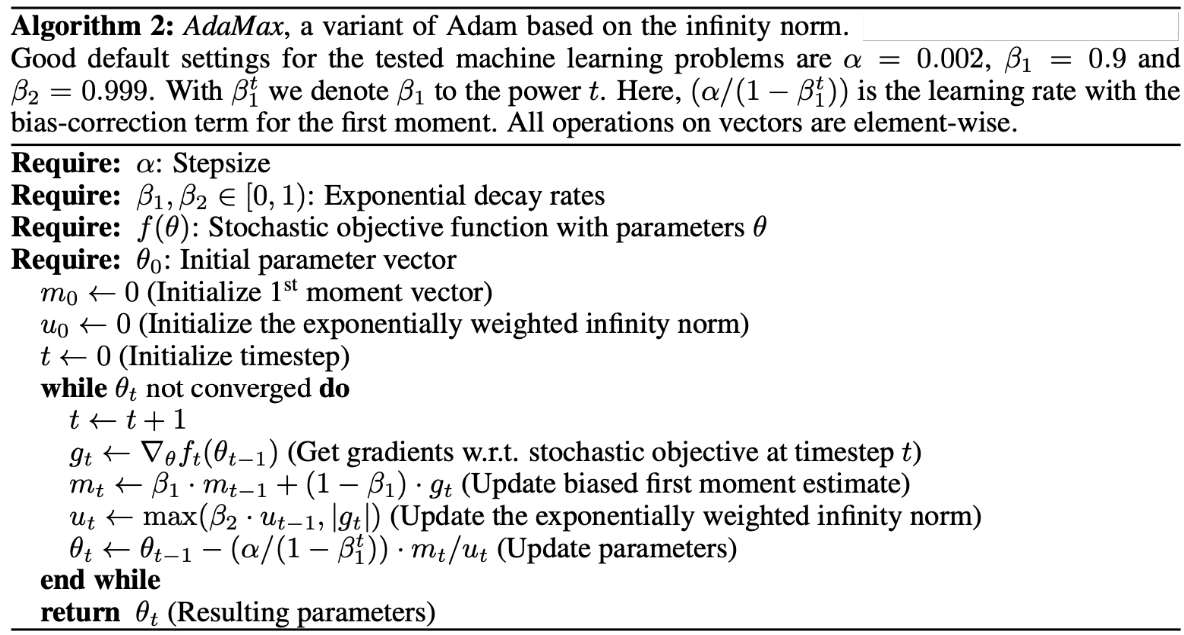
\includegraphics[scale=0.35]{images/h2}
\end{figure}

Lưu ý rằng thuật ngữ phân rã ở đây được tham số hoá là $\beta_2^p$ thay vì $\beta_2$. Nếu $p \rightarrow \infty$  và $u_t=\lim _{p \rightarrow \infty}\left(v_t\right)^{1 / p}$ thì
$$
\begin{aligned}
u_t=\lim _{p \rightarrow \infty}\left(v_t\right)^{1 / p} &=\lim _{p \rightarrow \infty}\left(\left(1-\beta_2^p\right) \sum_{i=1}^t \beta_2^{p(t-i)} \cdot\left|g_i\right|^p\right)^{1 / p} \\
&=\lim _{p \rightarrow \infty}\left(1-\beta_2^p\right)^{1 / p}\left(\sum_{i=1}^t \beta_2^{p(t-i)} \cdot\left|g_i\right|^p\right)^{1 / p} \\
&=\lim _{p \rightarrow \infty}\left(\sum_{i=1}^t \beta_2^{p(t-i)} \cdot\left|g_i\right|^p\right)^{1 / p} \\
&=\max \left(\beta_2^{t-1}\left|g_1\right|, \beta_2^{t-2}\left|g_2\right|, \ldots, \beta_2\left|g_{t-1}\right|,\left|g_t\right|\right)
\end{aligned}
$$
\subsection{Nadam}
Adam có thể được xem như là sự kết hợp của RMSprop và momentum vì nó sử dụng các trung bình trượt theo cấp số nhân (exponential moving averages) của bình phương gradient và gradient. Mặt khác, ta đã biết Nesterov accelerated gradient (NAG) giúp cho thuật toán hội tụ nhanh hơn so với momentum thông thường. Nadam (Nesterovaccelerated Adaptive Moment Estimation) là một thuật toán kết hợp Adam và NAG. Để phát triển Nadam, ta phải điều chỉnh giá trị momentum $m_t$ trong Adam. Đầu tiên, ta xem lại công thức cập nhật momentum
$$
\begin{aligned}
g_t &=\nabla \theta_t J\left(\theta_t\right), \\
m_t &=\gamma m_{t-1}+\eta g_t, \\
\theta_{t+1} &=\theta_t-m_t.
\end{aligned}
$$
Trong đó, $\nabla \theta_t J\left(\theta_t\right)$ là gradient của điểm trước đó, $m_t$ là momentum của điểm trước đó, $\gamma$ thường được chọn với giá trị $0.9, \eta$ là learning rate.
Mở rộng phương trình trên ta được
$$
\theta_{t+1}=\theta_t-\left(\gamma m_{t-1}+\eta g_t\right).
$$
Có thể thấy với momentum thông thường, lượng thay đổi là tổng của hai vector: momentum vector và gradient ở thời điểm hiện tại.
Với Nesterove momentum, lượng thay đổi là tổng của hai vector: momentum vector và gradient ở thời điểm được xấp xỉ là điểm tiếp theo. Ta có công thức của NAG
$$
\begin{aligned}
g_t &=\nabla \theta_t J\left(\theta_t-\gamma m_{t-1}\right), \\
m_t &=\gamma m_{t-1}+\eta g_t, \\
\theta_{t+1} &=\theta_t-m_t.
\end{aligned}
$$
Dozat đề xuất cải biến NAG như sau: Thay vì áp dụng momentum hai lần - một lần để cập nhật gradient $g_t$ và lần thứ hai để cập nhật $\theta_{t+1}$, chúng ta áp dụng trực tiếp momentum xấp xỉ điểm tiếp theo để cập nhật các tham số hiện tại
$$
\begin{aligned}
g_t &=\nabla \theta_t J\left(\theta_t\right), \\
m_t &=\gamma m_{t-1}+\eta g_t,\\
\theta_{t+1} &=\theta_t-\left(\gamma m_t+\eta g_t\right).
\end{aligned}
$$
Có thể thấy trong công thức trên, thay vì sử dụng vector momentum $m_{t-1}$ như trong phương pháp momentum, giờ ta sử dụng vector momentum $m_t$ để đi trước một bước.




\chapter{Thực nghiệm}

Trong chương này, em trình bày code để thực nghiệm thuật toán tối ưu Adam. Chi tiết quá trình này được thực hiện trong file notebook \url{https://github.com/nguyenquocduongqnu/Optimization_Theory_QNU}.
\section{Lập trình từ đầu cho thuật toán tối ưu Adam}
\section{Hồi quy logistic trên tập dữ liệu ung thư vú từ thư viện Sklearn sử dụng trình tối ưu theo thuật toán Adam}
\section{Thực nghiệm Adam và so sánh với các thuật toán cơ sở}
Các thuật toán Gradient Descent có rất nhiều vấn đề trong quá trình hội tụ, đặc biệt với những hàm số khó hội tụ tốt như hàm số có nhiều cực tiểu địa phương, nhiều điểm yên ngựa.
Để so sánh Adam đã giải quyết những vấn đề trên so với những giải thuật cơ sở ta tiến hành lấy một hàm số có tính chất như vậy để thử nghiệm
$$f(x)=\log \left(1+(|x|)^{2+s i n x}\right).$$
%%%%%%%%%%%%%%%%%%%%%%%%%%%%%%%%%%%%%%%
\newpage
\chapter*{KẾT LUẬN}
\fontsize{14pt}{14pt}\selectfont

Qua quá trình tìm hiểu, chúng ta có thể thấy rằng nhiều thuật toán tối ưu hóa dựa trên gradient descent đã được đưa ra và những thuật toán sau luôn được bổ sung hoàn thiện để giải quyết những tồn tại của thuật toán trước. RMSprop là một mở rộng của Adagrad với khả năng giải quyết vấn đề learning rate trở nên quá nhỏ. Sau đó, thuật toán Adam bổ sung thêm bias-correction và momentum vào RMSprop để mang lại hiệu năng tốt hơn, nó sử dụng các cập nhật gradient tỷ lệ với căn bậc hai của bình phương trung bình trượt các gradient trong quá khứ. Trong bài tiểu luận này, em đã thực hiện được một số công việc sau
\begin{itemize}
\item Giới thiệu tổng quan về tối ưu trong học sâu.
\item Giới thiệu tổng quan một số thuật toán làm nền tảng để nghiên cứu thuật toán tối ưu Adam.
\item Trình bày chi tiết bài báo gốc thuật toán tối ưu Adam và chứng minh thuật toán Adam có thể không hội tụ.
\item Thực nghiệm thuật toán Adam với mô hình hồi quy Logistic và so sánh với các thuật toán tối ưu khác.
\end{itemize}

\clearpage
\begin{thebibliography}{99}
	\addcontentsline{toc}{chapter}{TÀI LIỆU THAM KHẢO}
	\bibitem{1} Ian Goodfellow, Yoshua Bengio, Aaron Courville, \textit{Deep Learning}, MIT Press, 2016.
	\bibitem{2} Charu C. Aggarwal, \textit{Linear Algebra and Optimization for Machine Learning}, A Textbook-Springer, 2020.
	\bibitem{3} Aston Zhang, Zack C. Lipton, Mu Li, Alex J. Smola, \textit{Dive into Deep Learning}, \url{https://d2l.ai/}.
	\bibitem{4} Vũ Hữu Tiệp, \textit{Machine learning cơ bản}, Nhà xuất bản khoa học và kĩ thuật, 2019.
	\bibitem{5} Trần Trung Trực, \textit{Optimizer- Hiểu sâu về các thuật toán tối ưu ( GD,SGD,Adam,..)}, \url{https://viblo.asia/p/optimizer-hieu-sau-ve-cac-thuat-toan-toi-uu-gdsgdadam-Qbq5QQ9E5D8}.
	\bibitem{6} Sebastian ruder, \textit{\textit{An overview of gradient descent optimization algorithms}}, \url{https://ruder.io/optimizing-gradient-descent/index.html}.
	\bibitem{7} Diederik P. Kingma, Jimmy Lei Ba, \textit{Adam: A Method for Stochastic Optimization}, International Conference on Learning Representations, 2015.
	\bibitem{8} Sashank J.Reddi, Satyen Kate, Sanjiv Kumar, \textit{On the convergence of adam and
	beyond}, ICLR 2018.


\end{thebibliography}
\end{document}